\section{独立性}
设$A,B$是试验$E$的两事件,通常,事件$A$的发生对事件$B$发生的概率是有影响的,这将表现为$P(B\mid A)\neq P(B)$,只有当这种影响不存在时才会有$P(B\mid A)=P(B)$成立,我们将这种特性称为事件$A,B$独立,而作为独立的定义,我们援引\fancyref{fml:概率的乘法公式}
\begin{Equation}
    P(AB)=P(B\mid A)P(A)
\end{Equation}
由于$P(B\mid A)=P(B)$,应有
\begin{Equation}
    P(AB)=P(A)P(B)
\end{Equation}
我们用这个式子作为$A,B$的独立。
\begin{BoxDefinition}[独立性]
    设$A,B$是两事件,如果满足等式
    \begin{Equation}
        P(AB)=P(A)P(B)
    \end{Equation} 
    则称事件$A,B$ \uwave{相互独立},简称$A,B$ \uwave{独立}(Independence)。   
\end{BoxDefinition}
\begin{BoxProperty}[独立性与条件概率]
    设$A,B$是两独立事件,若$P(A)>0$,则分别有
    \begin{Equation}
        P(B\mid A)=P(B)
    \end{Equation}
\end{BoxProperty}
\begin{Proof}
    这是显然的,根据\fancyref{thm:贝叶斯定理}和\fancyref{def:独立性}
    \begin{Equation}*
        P(B\mid A)=\frac{P(AB)}{P(A)}=\frac{P(A)P(B)}{P(A)}=P(B)\qedhere
    \end{Equation}
\end{Proof}

\begin{BoxProperty}[独立性和互不相容]
    设$A,B$的两独立事件,则$A,B$必然不是互不相容的,反之亦然。
\end{BoxProperty}

\fancyref{ppt:独立性和互不相容}指出,独立性和互不相容性是无法同时成立的,这其实是很容易理解的,因为根据\fancyref{def:互斥事件},互不相容要求$A\cap B=\empty$,如果以概率形式表述,互不相容即要求$P(AB)=0$,而另外一方面,独立性要求$P(AB)=P(A)P(B)$,所以这两者显然是矛盾的。不过这里更想论述的是另一个问题,我们总是喜欢用文氏图的方式表述,现在的问题是,\empx{独立性在文氏图上如何表现}?因为首先,独立性肯定不是两个没有交集的圈,后者是互不相容的表现。独立性的事件在文氏图上肯定是有交集的,那它和普通的事件关系又有什么差异呢?实际情况是\cite{W3}\cite{W4},独立性并不能在文氏图上表现,因为,\empx{独立性是定量性质,文氏图是定性的表示手段},通常来说文氏图中的面积大小并不表示概率的大小,独立性则要求$P(AB)$恰好是$P(A)P(B)$,既不多,也不少,这种定量性,是文氏图是无法表示的。

但如果,我们要求文氏图的面积表征概率,那独立性就可以表示了,如\xref{fig:独立性}所示
\begin{Figure}[独立性]
    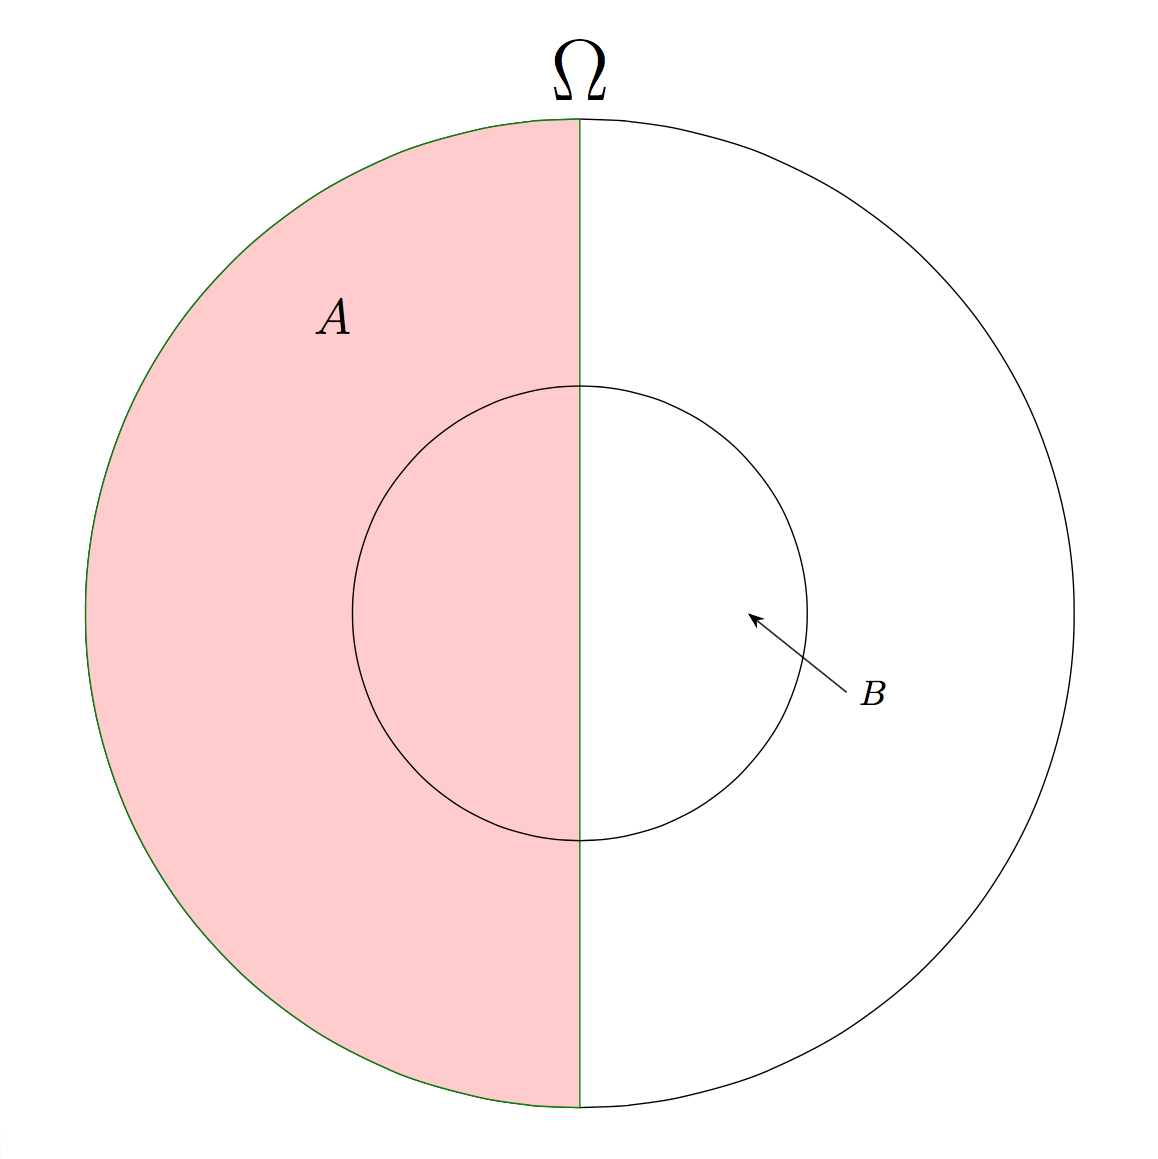
\includegraphics[width=6cm]{image/1.png}
    \vspace{0.25cm}
\end{Figure}

这里$B$是内圆,而$A$是红色的右半大圆,我们注意到,这两者占有全集$\Omega$的比例,与其各自在对方中的比例是相同的。例如,$B$在$\Omega$中,是半径较小的圆在一个半径较大的圆中,而另外一方面,$B$在$A$中,是半径较小的半圆在一个半径较大的半圆中。而类似的,$A$在$\Omega$中是一半,同时,$A$在$B$中也恰好是一半,这就形象的表现了条件概率与原概率相同的特点。

独立性的概念也可以推广到三个事件,设$A,B,C$是三个事件,若
\begin{Equation}
    \qquad\qquad
    P(AB)=P(A)P(B)\qquad
    P(BC)=P(B)P(C)\qquad
    P(CA)=P(C)P(A)
    \qquad\qquad
\end{Equation}
且
\begin{Equation}
    P(ABC)=P(A)P(B)P(C)
\end{Equation}
那就称$A,B,C$是独立的,由此亦可以推广至$n$个事件独立。